%%%%%%%%%%%%%%%%%%%%%%%%%%%%%%%%%%%%%%%%%%%%%%%%%%%%%%%%%%%%%%%%%%%%%%
% LaTeX Example: Project Report
%
% Source: http://www.howtotex.com
%
% Feel free to distribute this example, but please keep the referral
% to howtotex.com
% Date: March 2011 
% 
%%%%%%%%%%%%%%%%%%%%%%%%%%%%%%%%%%%%%%%%%%%%%%%%%%%%%%%%%%%%%%%%%%%%%%
% How to use writeLaTeX: 
%
% You edit the source code here on the left, and the preview on the
% right shows you the result within a few seconds.
%
% Bookmark this page and share the URL with your co-authors. They can
% edit at the same time!
%
% You can upload figures, bibliographies, custom classes and
% styles using the files menu.
%
% If you're new to LaTeX, the wikibook is a great place to start:
% http://en.wikibooks.org/wiki/LaTeX
%
%%%%%%%%%%%%%%%%%%%%%%%%%%%%%%%%%%%%%%%%%%%%%%%%%%%%%%%%%%%%%%%%%%%%%%
% Edit the title below to update the display in My Documents
%\title{Project Report}
%
%%% Preamble
\documentclass[paper=a4, fontsize=11pt]{scrartcl}
\usepackage[T1]{fontenc}
\usepackage{fourier}
\usepackage[utf8]{inputenc}
\usepackage[spanish]{babel}															% English language/hyphenation
\usepackage[protrusion=true,expansion=true]{microtype}	
\usepackage{amsmath,amsfonts,amsthm} % Math packages
\usepackage[pdftex]{graphicx}	
\usepackage{url}
\usepackage{hyperref}

%%% Custom sectioning
\usepackage{sectsty}
\allsectionsfont{\normalfont\scshape}


%%% Custom headers/footers (fancyhdr package)
\usepackage{fancyhdr}
\pagestyle{fancyplain}
\fancyhead{}											% No page header
\fancyfoot[L]{}											% Empty 
\fancyfoot[C]{}											% Empty
\fancyfoot[R]{\thepage}									% Pagenumbering
\renewcommand{\headrulewidth}{0pt}			% Remove header underlines
\renewcommand{\footrulewidth}{0pt}				% Remove footer underlines
\setlength{\headheight}{13.6pt}


%%% Equation and float numbering
\numberwithin{equation}{section}		% Equationnumbering: section.eq#
\numberwithin{figure}{section}			% Figurenumbering: section.fig#
\numberwithin{table}{section}				% Tablenumbering: section.tab#


% Custom colors
\usepackage{color}
\definecolor{deepblue}{rgb}{0,0,0.5}
\definecolor{deepred}{rgb}{0.6,0,0}
\definecolor{deepgreen}{rgb}{0,0.5,0}

\usepackage{listings}

% Python style for highlighting
\newcommand\pythonstyle{\lstset{
language=Python,
basicstyle=\ttm,
otherkeywords={self},             % Add keywords here
keywordstyle=\ttb\color{deepblue},
emph={MyClass,__init__},          % Custom highlighting
emphstyle=\ttb\color{deepred},    % Custom highlighting style
stringstyle=\color{deepgreen},
% frame=tb,                         % Any extra options here
showstringspaces=false            % 
}}


% Python environment
\lstnewenvironment{python}[1][]
{
\pythonstyle
\lstset{#1}
}
{}

% Python for external files
\newcommand\pythonexternal[2][]{{
\pythonstyle
\lstinputlisting[#1]{#2}}}

% Python for inline
\newcommand\pythoninline[1]{{\pythonstyle\lstinline!#1!}}

%%% Maketitle metadata
\newcommand{\horrule}[1]{\rule{\linewidth}{#1}} 	% Horizontal rule

\title{
		%\vspace{-1in} 	
		\usefont{OT1}{bch}{b}{n}
		\normalfont \normalsize \textsc{Universidad Católica de San Pablo \\
		Maestría en Ciencia de la Computación \\
        Sistemas Inteligentes} \\ [25pt]
		\horrule{0.5pt} \\[0.4cm]
		\huge Máquina de Vectores de Soporte (SVM) \\
		(CORRECCIÓN)\\
        Prof. Graciela Meza Lovón \\
		\horrule{2pt} \\[0.5cm]
}
\author{
		\normalfont 								\normalsize
        Palomino Paucar, Daniel Alfredo\\[-3pt]		\normalsize
        Noviembre 26, 2018 \\
        \url{https://bit.ly/2r7y556}
}
\date{}

%%% Begin document
\begin{document}
\maketitle

\newpage
\section{Preguntas de Teoría}
    

\textbf{Sea el conjunto $N = {((1,6),-1), ((4,9),-1), ((4,6),-1), ((5,1),1), ((9,1),1), ((0,3),1), ((2,2),-1), ((3,1),-1)}$ y el hiperplano $H_1$ definido anteriormente.}\\
    

    
\textbf{9.} Calcule la holgura de los ejemplos no separables.\\
    
    \textbf{Respuesta:}
    
    Dado que para los ejemplos no separables:
    
    $$\epsilon_i=1-y_{i}D(x_i)$$
    
    Se tendrá para los ejemplos no separables ${((0,3),1), ((2,2),-1), ((3,1),-1)}$:
    
    \begin{enumerate}
        \item $((0,3),\ 1)$: $\epsilon_i = 3.8284$
        \item $((2,2),-1)$: $\epsilon_i = 0.2929$
        \item $((3,1),-1)$: $\epsilon_i = 1.7071$
    \end{enumerate}

\newpage
\section{Preguntas de Investigación}

\section{Implementación}

\textbf{2.} Experimente y muestre resultados usando diferentes valores para los parámetros de los kernels: lineal, polinomial, gaussiano, y el parámetro $C$. Los resultados deben ser mostrados en el documento pdf.
    
    \textbf{Implementación:}
    
    Como no se ha incluído el dataset, he propuesto trabajar el presente ejercicio con el siguiente dataset (Iris Flower): \url{https://archive.ics.uci.edu/ml/machine-learning-databases/iris/iris.data}\\
    
    \textbf{Lectura de Dataset}
    
    \begin{python}
    import numpy as np  
    import matplotlib.pyplot as plt  
    import pandas as pd
    
    url = "https://archive.ics.uci.edu/ml/machine-learning-databases"
          "/iris/iris.data"
    # Asignar columnas al Dataset para su posterior lectura
    colnames = ['sepal-length', 'sepal-width', 
                'petal-length', 'petal-width', 'Class']
    # Lectura del Dataset usando pandas
    irisdata = pd.read_csv(url, names=colnames)
    \end{python}
    
    \textbf{Exploración de Datos}
    
    \begin{python}
    # Descripción del Dataset
    bankdata.head()
    \end{python}
    
    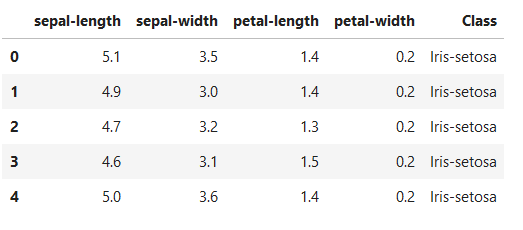
\includegraphics[scale=0.8]{df2_head}
    \newpage
    \textbf{Preprocesamiento}
    
    \begin{python}
    # Separación de las columnas del dataset para crear los valores de entrada
    # y el valor de salida
    X = irisdata.drop('Class', axis=1)  
    y = irisdata['Class'] 
    # Separación del dataset en valores de entranemiento y testeo
    from sklearn.model_selection import train_test_split  
    X_train, X_test, y_train, y_test = train_test_split(X, y, test_size = 0.20) 
    \end{python}
    
    \textbf{Lineal con C=0.5}
    
    \textbf{Entrenamiento}
    
    \begin{python}
    from sklearn.svm import SVC
    # Elección del Kernel: linear Y parámetro C=0.5
    svclassifier = SVC(kernel='linear', C=0.5)
    # Ejecución del entrenamiento
    svclassifier.fit(X_train, y_train)
    \end{python}
    
    \textbf{Predicción y Validación}
    
    \begin{python}
    # Predicción usando los valores de testeo
    y_pred = svclassifier.predict(X_test)
    from sklearn.metrics import classification_report, confusion_matrix
    # Creación de la matriz de confusión
    print(confusion_matrix(y_test,y_pred))
    # Creación de reporte de resultados
    print(classification_report(y_test,y_pred))
    \end{python}
    
    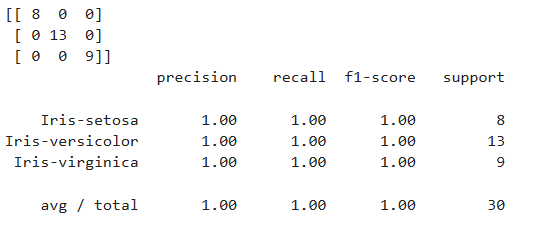
\includegraphics[scale=0.8]{lineal_c_05}
    \newpage
    
    \textbf{Lineal con C=1.0}
    
    \textbf{Entrenamiento}
    
    \begin{python}
    from sklearn.svm import SVC
    # Elección del Kernel: linear Y parámetro C=1.0
    svclassifier = SVC(kernel='linear', C=1.0)
    # Ejecución del entrenamiento
    svclassifier.fit(X_train, y_train)
    \end{python}
    
    \textbf{Predicción y Validación}
    
    \begin{python}
    # Predicción usando los valores de testeo
    y_pred = svclassifier.predict(X_test)
    from sklearn.metrics import classification_report, confusion_matrix
    # Creación de la matriz de confusión
    print(confusion_matrix(y_test,y_pred))
    # Creación de reporte de resultados
    print(classification_report(y_test,y_pred))
    \end{python}
    
    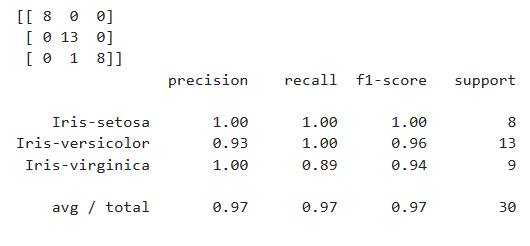
\includegraphics[scale=0.8]{lineal_c_10}
    \newpage
    
    \textbf{Lineal con C=2.0}
    
    \textbf{Entrenamiento}
    
    \begin{python}
    from sklearn.svm import SVC
    # Elección del Kernel: linear Y parámetro C=2.0
    svclassifier = SVC(kernel='linear', C=2.0)
    # Ejecución del entrenamiento
    svclassifier.fit(X_train, y_train)
    \end{python}
    
    \textbf{Predicción y Validación}
    
    \begin{python}
    # Predicción usando los valores de testeo
    y_pred = svclassifier.predict(X_test)
    from sklearn.metrics import classification_report, confusion_matrix
    # Creación de la matriz de confusión
    print(confusion_matrix(y_test,y_pred))
    # Creación de reporte de resultados
    print(classification_report(y_test,y_pred))
    \end{python}
    
    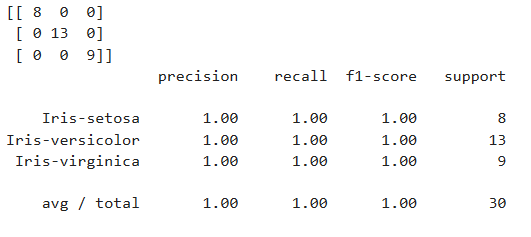
\includegraphics[scale=0.8]{lineal_c_20}
    \newpage
    
    \textbf{Lineal con C=5.0}
    
    \textbf{Entrenamiento}
    
    \begin{python}
    from sklearn.svm import SVC
    # Elección del Kernel: linear Y parámetro C=5.0
    svclassifier = SVC(kernel='linear', C=5.0)
    # Ejecución del entrenamiento
    svclassifier.fit(X_train, y_train)
    \end{python}
    
    \textbf{Predicción y Validación}
    
    \begin{python}
    # Predicción usando los valores de testeo
    y_pred = svclassifier.predict(X_test)
    from sklearn.metrics import classification_report, confusion_matrix
    # Creación de la matriz de confusión
    print(confusion_matrix(y_test,y_pred))
    # Creación de reporte de resultados
    print(classification_report(y_test,y_pred))
    \end{python}
    
    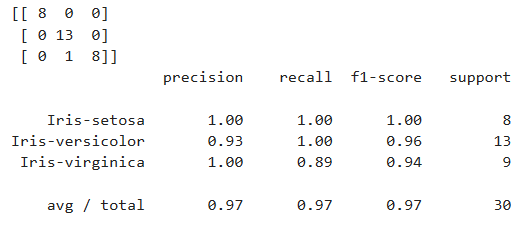
\includegraphics[scale=0.8]{lineal_c_50}
    \newpage
    
    \textbf{Polinomial con C=0.5}
    
    \textbf{Entrenamiento}
    
    \begin{python}
    from sklearn.svm import SVC
    # Elección del Kernel: poly Y parámetro C=0.5
    svclassifier = SVC(kernel='poly', degree=8, C=0.5)
    # Ejecución del entrenamiento
    svclassifier.fit(X_train, y_train)
    \end{python}
    
    \textbf{Predicción y Validación}
    
    \begin{python}
    # Predicción usando los valores de testeo
    y_pred = svclassifier.predict(X_test)
    from sklearn.metrics import classification_report, confusion_matrix
    # Creación de la matriz de confusión
    print(confusion_matrix(y_test,y_pred))
    # Creación de reporte de resultados
    print(classification_report(y_test,y_pred))
    \end{python}
    
    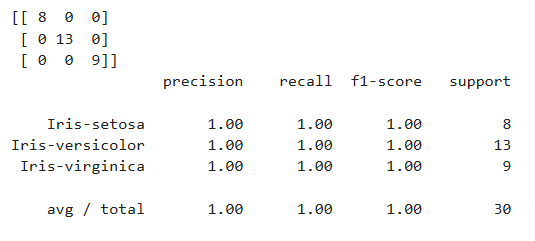
\includegraphics[scale=0.8]{polynomial_c_05}
    \newpage
    
    \textbf{Polinomial con C=1.0}
    
    \textbf{Entrenamiento}
    
    \begin{python}
    from sklearn.svm import SVC
    # Elección del Kernel: poly Y parámetro C=1.0
    svclassifier = SVC(kernel='poly', degree=8, C=1.0)
    # Ejecución del entrenamiento
    svclassifier.fit(X_train, y_train)
    \end{python}
    
    \textbf{Predicción y Validación}
    
    \begin{python}
    # Predicción usando los valores de testeo
    y_pred = svclassifier.predict(X_test)
    from sklearn.metrics import classification_report, confusion_matrix
    # Creación de la matriz de confusión
    print(confusion_matrix(y_test,y_pred))
    # Creación de reporte de resultados
    print(classification_report(y_test,y_pred))
    \end{python}
    
    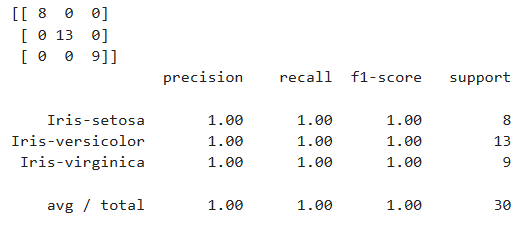
\includegraphics[scale=0.8]{polynomial_c_10}
    \newpage
    
    \textbf{Polinomial con C=2.0}
    
    \textbf{Entrenamiento}
    
    \begin{python}
    from sklearn.svm import SVC
    # Elección del Kernel: poly Y parámetro C=2.0
    svclassifier = SVC(kernel='poly', degree=8, C=2.0)
    # Ejecución del entrenamiento
    svclassifier.fit(X_train, y_train)
    \end{python}
    
    \textbf{Predicción y Validación}
    
    \begin{python}
    # Predicción usando los valores de testeo
    y_pred = svclassifier.predict(X_test)
    from sklearn.metrics import classification_report, confusion_matrix
    # Creación de la matriz de confusión
    print(confusion_matrix(y_test,y_pred))
    # Creación de reporte de resultados
    print(classification_report(y_test,y_pred))
    \end{python}
    
    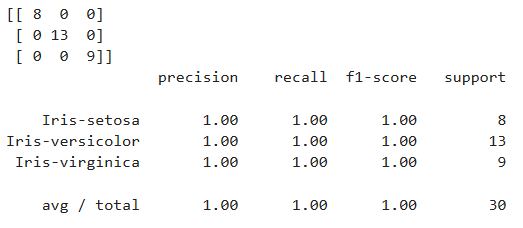
\includegraphics[scale=0.8]{polynomial_c_20}
    \newpage
    
    \textbf{Polinomial con C=5.0}
    
    \textbf{Entrenamiento}
    
    \begin{python}
    from sklearn.svm import SVC
    # Elección del Kernel: poly Y parámetro C=5.0
    svclassifier = SVC(kernel='poly', degree=8, C=5.0)
    # Ejecución del entrenamiento
    svclassifier.fit(X_train, y_train)
    \end{python}
    
    \textbf{Predicción y Validación}
    
    \begin{python}
    # Predicción usando los valores de testeo
    y_pred = svclassifier.predict(X_test)
    from sklearn.metrics import classification_report, confusion_matrix
    # Creación de la matriz de confusión
    print(confusion_matrix(y_test,y_pred))
    # Creación de reporte de resultados
    print(classification_report(y_test,y_pred))
    \end{python}
    
    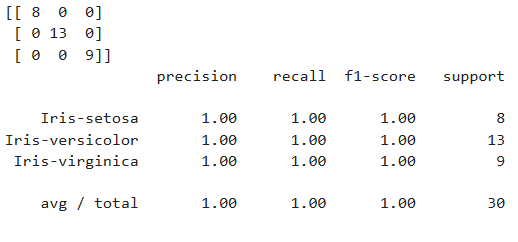
\includegraphics[scale=0.8]{polynomial_c_50}
    \newpage
    
    \textbf{Gaussiano con C=0.5}
    
    \textbf{Entrenamiento}
    
    \begin{python}
    from sklearn.svm import SVC
    # Elección del Kernel: rbf y C=0.5
    svclassifier = SVC(kernel='rbf', C=0.5)
    # Ejecución del entrenamiento
    svclassifier.fit(X_train, y_train)
    \end{python}

    \textbf{Predicción y Validación}
    
    \begin{python}
    # Predicción usando los valores de testeo
    y_pred = svclassifier.predict(X_test)
    from sklearn.metrics import classification_report, confusion_matrix
    # Creación de la matriz de confusión
    print(confusion_matrix(y_test,y_pred))
    # Creación de reporte de resultados
    print(classification_report(y_test,y_pred))
    \end{python}
    
    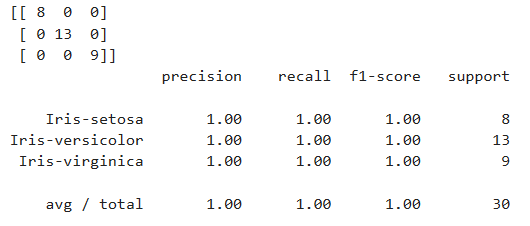
\includegraphics[scale=0.8]{gaussiano_c_05}
    \newpage
    
     \textbf{Gaussiano con C=1.0}
    
    \textbf{Entrenamiento}
    
    \begin{python}
    from sklearn.svm import SVC
    # Elección del Kernel: rbf y C=1.0
    svclassifier = SVC(kernel='rbf', C=1.0)
    # Ejecución del entrenamiento
    svclassifier.fit(X_train, y_train)
    \end{python}

    \textbf{Predicción y Validación}
    
    \begin{python}
    # Predicción usando los valores de testeo
    y_pred = svclassifier.predict(X_test)
    from sklearn.metrics import classification_report, confusion_matrix
    # Creación de la matriz de confusión
    print(confusion_matrix(y_test,y_pred))
    # Creación de reporte de resultados
    print(classification_report(y_test,y_pred))
    \end{python}
    
    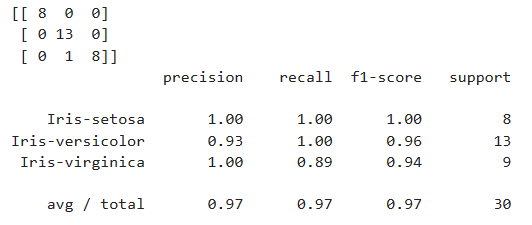
\includegraphics[scale=0.8]{gaussiano_c_10}
    \newpage
    
     \textbf{Gaussiano con C=2.0}
    
    \textbf{Entrenamiento}
    
    \begin{python}
    from sklearn.svm import SVC
    # Elección del Kernel: rbf y C=2.0
    svclassifier = SVC(kernel='rbf', C=2.0)
    # Ejecución del entrenamiento
    svclassifier.fit(X_train, y_train)
    \end{python}

    \textbf{Predicción y Validación}
    
    \begin{python}
    # Predicción usando los valores de testeo
    y_pred = svclassifier.predict(X_test)
    from sklearn.metrics import classification_report, confusion_matrix
    # Creación de la matriz de confusión
    print(confusion_matrix(y_test,y_pred))
    # Creación de reporte de resultados
    print(classification_report(y_test,y_pred))
    \end{python}
    
    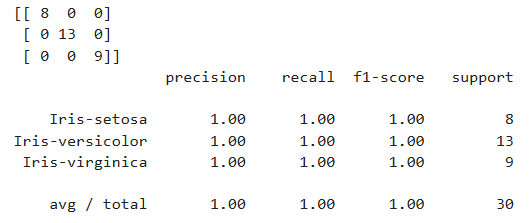
\includegraphics[scale=0.8]{gaussiano_c_20}
    \newpage
    
     \textbf{Gaussiano con C=5.0}
    
    \textbf{Entrenamiento}
    
    \begin{python}
    from sklearn.svm import SVC
    # Elección del Kernel: rbf y C=5.0
    svclassifier = SVC(kernel='rbf', C=5.0)
    # Ejecución del entrenamiento
    svclassifier.fit(X_train, y_train)
    \end{python}

    \textbf{Predicción y Validación}
    
    \begin{python}
    # Predicción usando los valores de testeo
    y_pred = svclassifier.predict(X_test)
    from sklearn.metrics import classification_report, confusion_matrix
    # Creación de la matriz de confusión
    print(confusion_matrix(y_test,y_pred))
    # Creación de reporte de resultados
    print(classification_report(y_test,y_pred))
    \end{python}
    
    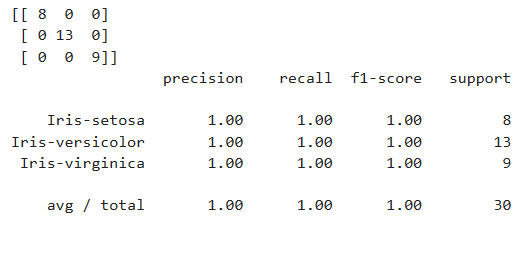
\includegraphics[scale=0.8]{gaussiano_c_50}
    \newpage
    
    \textbf{3.} Dentro de la sección de Implementación incluya una subsección donde indique las instrucciones para ejecutar el código.
    
    \textbf{Implementación:}
    
    La presente implementación ha sido realizada en python 3.6 usando anaconda y jupyter-lab como herramientas de virtualización y visualización.
    
    El notebook desarrollado que incluye todos los pasos descritos, así como los datasets, ha sido publicado en mi cuenta de github:\\
    
    \url{https://github.com/dpalominop/SistemasInteligentes/blob/master/semana7/homework/svm.ipynb}

%%% End document
\end{document}